
%(BEGIN_QUESTION)
% Copyright 2007, Tony R. Kuphaldt, released under the Creative Commons Attribution License (v 1.0)
% This means you may do almost anything with this work of mine, so long as you give me proper credit

The {\it pH value} of an aqueous (water-based) solution can be a challenging process variable to control.  When a caustic substance (high pH) is added to an acidic solution (low pH), the pH value of that solution will rise accordingly, but it often rises in a very non-linear way.  If we are adding a strongly concentrated caustic to a strongly concentrated acid, what we initially see is a mild increase in pH, followed by a very rapid rise in pH, followed by another mild increase.  This is called a {\it titration curve}, an example shown in this graph:

$$\includegraphics[width=15.5cm]{i01695x01.eps}$$

First, identify how the calculus concept of the {\it derivative} applies to a titration curve (i.e. what does ``derivative'' mean in this context?) and how you would write a mathematically-correct expression for this derivative.  Next, identify where on this titration curve it will be ``easiest'' for an automatic control system to regulate the pH value of the liquid solution, and where it will be the most challenging (and also why!).

\vskip 20pt \vbox{\hrule \hbox{\strut \vrule{} {\bf Suggestions for Socratic discussion} \vrule} \hrule}

\begin{itemize}
\item{} A relevant concept to consider in this scenario is the idea of {\it process gain}: how responsive a process variable (i.e. the solution's pH value in this case) will be to changes in the manipulated variable (i.e. the amount of caustic material the control system adds to the solution).  Where along the titration curve is the process gain greatest?  Where is the process gain minimal?
\item{} How do you think the gain of a proportional loop controller should be set in relation to the gain of the process it is tasked with controlling?  For example, if we wished to control pH at a point on the titration curve where the process gain is very high, should the controller be ``tuned'' with a high amount of gain or a low amount of gain?  Why?
\end{itemize}

\underbar{file i01695}
%(END_QUESTION)





%(BEGIN_ANSWER)

A mathematically-correct expression for this derivative:

$${d \hbox{pH} \over dm}$$

%(END_ANSWER)





%(BEGIN_NOTES)

``Derivative'' in this context means the ratio of pH change to change in reagant addition.  The system will be difficult to control whenever the slope is very steep (in the middle) or where the slope is nearly level.  At the steep point, the system gain will be high and loop oscillations may result.  At the level points, large changes in reagant feed will be necessary to effect modest changes in pH, making the loop sluggish to respond to setpoint and load changes.

%INDEX% Chemistry, pH: titration curve
%INDEX% Process: water pH neutralization (generic)

%(END_NOTES)


